\section{Distribución conjunta de un vector aleatorio}


\subsection{Modelos para vectores aleatorios}

Cuando estudiamos experimentos aleatorios podemos tener interes en la variación conjunta de dos o más características o variables aleatorias del mismo. \\
Estas agrupaciones de varias características se conocen como vectores aleatorios. 
Por tanto el conjunto de vectores aleatorios posibles será ahora un subconjunto de 
\(\mathbb{R}^n\), siendo n la dimensión del vector aleatorio, osea el número de caracteristicas 
estudiadas. \\
Ademas de distribuciones discretas, continuas y mixtas, es posible encontrar algunas que no entre en ninguno
de los anteriores grupos, pero nuestro estudio se centrará en las distribuciones discretas y continuas. \\ \\

Llamaremos \textit{distribución conjunta del vector} al modelo probabilistico asociado a un vector aleatorio.
Un vector aleatorio se describe como \(X = (X_1, ... , X_n)\) siendo el resultado de la consideración conjunta de variables aleatorioas. 
Llamaremos \textit{distribución marginal} \(X_i\) a la distribución asociada a la caracteristica descrita por dicha variable por separado. \\
Es posible crear un vector mediante otros vectores de la forma \(X = (X_a, X_b)\); en estos casos, para referirnos a la distribución de \(X_a\) tambíen hablatemos de la \textit{Distribución marginal} de \(X_a\).

\subsection{Vectores aleatorios discretos}

Los modelos multivariantes discretos (modelos para vectores aleatorios) reproducen las
características de los modelos univariantes: \\
El conjunto de los valores posibles de \(X = (X_1,...,X_n)\) es un conjunto discreto
de elementos de \(\mathbb{R}^n\) y la probabilidad se concentra en esos elementos. Los
sucesos no elementales se calculan mediante las sumas de los elementales. \\
Emplearemos la notación \(X_1 = x_1, ...,  X_n = x_n\) para referirnos al suceso 
consistente en el que el vector aleatorio \(X = (X_1, ...,X_n)\) toma el valor 
\(x = (x_1, ..., x_n)\). De forma analoga, \((X_1 \in A_1, ..., X_n \in A_n)\) denota
el suceso consistente en que el valor de \(X\) es un elemento de \(A_1 \times ... \times A_n\). Es inmediato entonces
\[(X_1 \in A_1, ..., X_n \in A_n) = (X_1 \in A_1) \cap ... \cap (X_n \in A_n)\] \\
\\
A la función 
\[p(x_1, ..., x_n) = P(X_1 = x_1, ..., X_n = x_n), \qquad (x_1, ..., x_n) \in \mathbb{R}^n\]
la llamaremos \textit{función de masa de probabilidad conjunta} del vector \(X\).

\newpage

Con esta notación los modelos probabilísticos para vectores aleatorios discretos pueden
resumirse de la siguiente forma: \\ \\
\(X = (X_1, ..., X_n), \quad \Omega = \{ x^1, x^2, ..., x^i, ... \}, \quad x^i = (x^i_1, ..., x^i_n) \in \mathbb{R}^n\) \\
\(P(X_1 = x_1, ..., X_n = x_n) = p(x_1, ..., x_n);\) \\
\(p(x_1, ..., x_n) \geq 0, \quad \displaystyle\sum_{(x_1, ..., x_n) \in \Omega} p(x_1, ..., x_n) = 1\) \\ \\
\[P((X_1, ..., X_n) \in A) = P\left( \displaystyle\bigcup_{(x_1, ..., x_m) \in A} (X_1 = x_1, ..., X_n = x_n) \right) = \displaystyle\sum_{(x_1, ..., x_n) \in A} p(x_1, ..., x_n)\] \\

\subsection{Distribución conjunta de un vector aleatorio bidimensional}

Dadas \(X\) e \(Y\) dos variables aleatorias definidas sobre el mismo espacio muestral
\(\Omega\), la \qquad aplicación \((X,Y):\Omega \to \mathbb{R}^2\) es un vector
aleatorio bidimensional. \\
La distribución que describe simultáneamente el comportamiento de \(X\) e \(Y\) se 
llama \textit{distribución de probabilidad conjunta}. \\ \\
Dado un vector aleatorio \((X, Y)\) y dados \(x,y \in \mathbb{R}\), la \textit{función
de distribución conjunta} de \((X, Y)\) evaluada en \((x, y)\) se define como:
\[F_{X, Y}(x, y) = P(X \leq x, Y \leq y) = P((X \leq x) \cap (Y \leq y))\]
Esta función es útil principalmente en los casos continuos y mixtos.

\subsection{Vectores aleatorios discretos}

Dadas \(X\) e \(Y\) dos variables aleatorias discretas, el vector \((X, Y)\) será 
discreto y tiene \textit{función de probabilidad conjunta} 
\[p(x, y) = P(X = x, Y = y)\] \\
Por tanto tenemos las siguientes propiedades
\begin{enumerate}
    \item \(p(x, y) \geq 0\)
    \item \(\sum_{x}\sum_{y} p(x, y) = 1\)
\end{enumerate}
y una \textit{función de distribución conjunta}
\[F(x_{0}, y_{0}) = P(X \leq x_0, Y \leq y_0) = \sum_{x \leq x_0} \sum_{y \leq y_0} p(x, y)\]

\newpage

\begin{theorem}
    Consideremos el experimento aleatorio consistente en seleccionar al azar y sin reemplazamiento dos números del conjunto \(\{1, 2, 3, 4, 5, 6, 7, 8 \}\). Centremos nuestra atención en el vector aleatorio \((X, Y)\) en el que \(X\) es el mayor número elegido e \(Y\) es el menor. 
    Los posibles valores de \((X, Y)\) son los pares de números enteros \((i, j)\) que verifican \(1 \leq j < i \leq 8\). Si \((i, j)\) verifica esas condiciones entonces
    \[P(X = i, Y = j) = \frac{1}{\binom{8}{2}} = \frac{1}{28}\]
    (el experimento consiste, esencialmente, en escoger una subpoblación de tamaño 2 de una población con 8 elementos). \\
    A menudo es conveniente recoger en una tabla de doble entrada la función de masa de probabilidad de un vector aleatorio bidimensional. La tabla correspondiente a este ejemplo es la siguiente:
    \begin{center}
    \begin{tabular}{|l|ccccccc|}
    \hline
    \diagbox{X}{Y} & 1 & 2 & 3 & 4 & 5 & 6 & 7 \\
        \hline
        2 & \(\frac{1}{28}\) & 0 & 0 & 0 & 0 & 0 & 0 \\
        3 & \(\frac{1}{28}\) & \(\frac{1}{28}\) & 0 & 0 & 0 & 0 & 0 \\
        4 & \(\frac{1}{28}\) & \(\frac{1}{28}\) & \(\frac{1}{28}\) & 0 & 0 & 0 & 0 \\
        5 & \(\frac{1}{28}\) & \(\frac{1}{28}\) & \(\frac{1}{28}\) & \(\frac{1}{28}\) & 0 & 0 & 0 \\
        6 & \(\frac{1}{28}\) & \(\frac{1}{28}\) & \(\frac{1}{28}\) & \(\frac{1}{28}\) & \(\frac{1}{28}\) & 0 & 0 \\
        7 & \(\frac{1}{28}\) & \(\frac{1}{28}\) & \(\frac{1}{28}\) & \(\frac{1}{28}\) & \(\frac{1}{28}\) & \(\frac{1}{28}\) & 0 \\
        7 & \(\frac{1}{28}\) & \(\frac{1}{28}\) & \(\frac{1}{28}\) & \(\frac{1}{28}\) & \(\frac{1}{28}\) & \(\frac{1}{28}\) & \(\frac{1}{28}\) \\
        \hline
    \end{tabular} 
    \end{center}
    A partir de la función masa podemos calcular la probabilidad de cualquier otro suceso relacionado con \((X, Y)\). Por ejemplo, si \(A\) es el suceso "la diferencia entre los dos números elegidos es menor que 5", entonces
    \[P((X, Y) \in A) = P(X - Y < 5) = \displaystyle\sum_{(i, j)\in A}p(i, j)\]
    es decir, que \(P(X - Y < 5\) se calcula sumando los valores de la función de masa de probabilidad sombreados en la siguiente tabla
    \begin{center}
    \begin{tabular}{|l|ccccccc|}
    \hline
    \diagbox{X}{Y} & 1 & 2 & 3 & 4 & 5 & 6 & 7 \\
        \hline
        2 & \colorbox{gray}{\textcolor{white}{\(\frac{1}{28}\)}} & 0 & 0 & 0 & 0 & 0 & 0 \\
        3 & \colorbox{gray}{\textcolor{white}{\(\frac{1}{28}\)}} & \colorbox{gray}{\textcolor{white}{\(\frac{1}{28}\)}} & 0 & 0 & 0 & 0 & 0 \\
        4 & \colorbox{gray}{\textcolor{white}{\(\frac{1}{28}\)}} & \colorbox{gray}{\textcolor{white}{\(\frac{1}{28}\)}} & \colorbox{gray}{\textcolor{white}{\(\frac{1}{28}\)}} & 0 & 0 & 0 & 0 \\
        5 & \colorbox{gray}{\textcolor{white}{\(\frac{1}{28}\)}} & \colorbox{gray}{\textcolor{white}{\(\frac{1}{28}\)}} & \colorbox{gray}{\textcolor{white}{\(\frac{1}{28}\)}} & \colorbox{gray}{\textcolor{white}{\(\frac{1}{28}\)}} & 0 & 0 & 0 \\
        6 & \(\frac{1}{28}\) & \colorbox{gray}{\textcolor{white}{\(\frac{1}{28}\)}} & \colorbox{gray}{\textcolor{white}{\(\frac{1}{28}\)}} & \colorbox{gray}{\textcolor{white}{\(\frac{1}{28}\)}} & \colorbox{gray}{\textcolor{white}{\(\frac{1}{28}\)}} & 0 & 0 \\
        7 & \(\frac{1}{28}\) & \(\frac{1}{28}\) & \colorbox{gray}{\textcolor{white}{\(\frac{1}{28}\)}} & \colorbox{gray}{\textcolor{white}{\(\frac{1}{28}\)}} & \colorbox{gray}{\textcolor{white}{\(\frac{1}{28}\)}} & \colorbox{gray}{\textcolor{white}{\(\frac{1}{28}\)}} & 0 \\
        7 & \(\frac{1}{28}\) & \(\frac{1}{28}\) & \(\frac{1}{28}\) & \colorbox{gray}{\textcolor{white}{\(\frac{1}{28}\)}} & \colorbox{gray}{\textcolor{white}{\(\frac{1}{28}\)}} & \colorbox{gray}{\textcolor{white}{\(\frac{1}{28}\)}} & \colorbox{gray}{\textcolor{white}{\(\frac{1}{28}\)}} \\
        \hline
    \end{tabular} 
    \end{center}
    Por lo tanto \(P(X - Y < 5) = \frac{22}{28} \approx 0,7857\)
\end{theorem}

\subsection{Vectores aleatorios continuos}

Diremos que el vector aleatorio \(X = (X_1, ..., X_n)\) es continuo y con 
función de densidad \(f(x_1, ..., x_n)\) si las probabilidades de los
sucesos de interés dentro del modelo se calculan segun la regla
\[P(X \in A) = \int_A f(x_1, ..., x_n)dx_1 \dotsi dx_n\]
Para que la anterior expresión defina un modelo probabilistico correcto
la función \(f\) debe verificar las siguientes condiciones
\begin{enumerate}
    \item \(f(x_1, ..., x_n) \geq 0, \qquad (x_1, ..., x_n) \in \Omega \subset \mathbb{R}^n\)
    \item \(\int_\Omega f(x_1, ..., x_n) dx_1 \dotsi dx_n = 1\)
\end{enumerate}
donde \(\Omega\), el conjunto de valores posibles de \(X\), es subconjunto
de \(\mathbb{R}^n\).
\subsubsection{Vector aleatorio continuo bidimensional}
Dados \(X\) e \(Y\) dos variables aleatorias continuas, el vector 
aleatorio \((X, Y)\) será contiuo y tiene \textit{función de densidad 
conjunta} \(f(x, y)\) que satisface
\begin{enumerate}
    \item \(f(x, y) \geq 0;\)
    \item \(\int\int f(x, y)dx dy = 1\)
\end{enumerate}
y una \textit{función de distribución conjunta} descrita como
\[F(x_0, y_0) ) P(X \leq x_0, Y \leq y_0) =  \int_{-\infty}^{x_0}\int_{-\infty}^{y_0} f(x, y)dy dx\]
Para calcular la probabilidad de que un suceso esté entre dos valores \((a, c)\) y \((b, d)\) tenemos que
\[P(a \leq X \leq b, c \leq Y \leq d) = \int_{a}^{b}\int_{c}^{d}f(x, y)dydx\]
\[F(x, y) = \int_{-\infty}^{x}\int_{-\infty}^{y} f(x, y)dydx\]
y ademas
\[f(x, y) = \frac{\delta^2}{\delta x\delta y}F(x, y)\]

\newpage

Aquí se pueden ver algunos ejemplos de funciones de densidad variables. El
analisis de la probabilidad consiste en calcular el volumen encerrado
bajo la superficie.
\vspace*{\fill}
	\begin{figure}[htbp]
        \center
        \includegraphics[scale=0.8]{img/FunciónDensidadBivariable.png}
        \caption{Una función de densidad bivariable}
    \end{figure}
\vspace*{\fill}
\vspace*{\fill}
    \begin{figure}[htbp]
        \center
        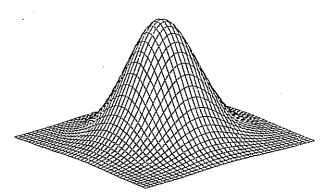
\includegraphics[scale=1]{img/NormalBivariable.png}
        \caption{Densidad normal bivariable}
    \end{figure}
\vspace*{\fill}

\newpage

\begin{theorem}
    Consideremos el experimento consistente en seleccionar un punto al azar en un círculo de radio unidad 
    (suponemos centrado en \((0, 0)\)). Llamaremos \(X\) e \(Y\) a la abcisa y a la ordenada del punto elegido. 
    La elección puramente al azar se puede modelizar con al función de densidad
    
    \[f(x, y) = \left\{
        \begin{array}{rcr}
            \frac{1}{\pi}   & si    & x^2 + y^2 \leq 1 \\
            0               & si    & x^2 + y^2 > 1
        \end{array}
    \right\}\]

    Esta función es una función de densidad. Fácilmente comprobamos que su integral es uno:

    \[\int_{\{(x, y) \big{/} x^2 + y^2 \leq 1\}} f(x, y)dxdy = \int_{-1}^{1} \left(\int_{-\sqrt{1 - x^2}}^{\sqrt{1 - x^2}} \frac{1}{\pi}dy\right)dx =\]
    \[=\frac{1}{\pi}\int_{-1}^{1} 2\sqrt{1 - x^2}dx = \frac{\pi}{\pi} = 1\]

    El cálculo de probabilidades dentro de este modelo se efectúa integrando la función de densidad en la región adecuada. 
    Consideremos los sucesos $A$ = \textit{"el punto elegido dista del origen menos de 0.5 unidades"} y $B$ = \textit{"la abcisa del 
    punto elegido está dentro del intervalo $(0.3, 0.8)$"}.
    
    \[P((X, Y) \in A) = P(X^2 + Y^2 < 0.5^2) = \int_{\{(x, y) \big{/} x^2 + y^2 < 0.25\}} f(x, y)dxdy =\]
    \[= \int_{-0.5}^{0.5} \left(\int_{-\sqrt{0.25 - x^2}}^{\sqrt{0.25 - x^2}} \frac{1}{\pi}dy\right)dx = \frac{1}{\pi}\int_{-0.5}^{0.5} 2\sqrt{0.25 - x^2}dx = \frac{\pi}{4\pi} = 0.25\]

    \[ P((X, Y) \in B) = P(0.3 < X < 0.8) = \int_{\{ (x, y) \big{/} 0.3 < x < 0.8 \}} f(x, y)dxdy = \]
    \[ = \int_{0.3}^{0.8} \left( \int_{-\sqrt{1 - x^2}}^{\sqrt{1 - x^2}} \frac{1}{\pi}dy \right) dx = \frac{1}{\pi} \int_{0.3}^{0.8} 2\sqrt{1 - x^2} dx = \]
    \[ \frac{1}{\pi} \left[ \arcsin x + x\sqrt{1 - x^2} \right]_{x = 0.3}^{x = 0.8} \approx 0.2599 \]

\end{theorem}

\begin{figure}[htbp]
    \center
    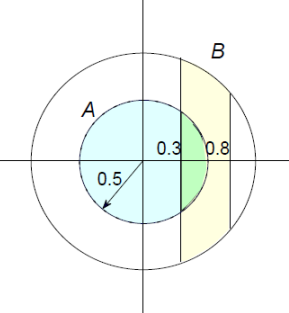
\includegraphics[scale=0.6]{img/Ejemplo2.png}
    \caption{Circunferencia de radio unidad y los conjuntos A y B}
\end{figure}
